% Preamble
\documentclass[a4paper, 12pt]{article}
\usepackage[margin=1in]{geometry} % Set margin
\usepackage{pdfpages} % Insert pdf pages
\usepackage{amssymb,amsmath,amsthm, amsfonts} % Math libraries

% Custom commands
\newcommand{\sub}[1]{\subsection{\underline{#1}}}
\newcommand{\subsub}[1]{\subsubsection{\underline{#1}}}
\newcommand{\?}{\stackrel{?}{=}}
\newcommand{\R}{\ensuremath{\mathbb{R}}}
\newcommand{\F}{\ensuremath{\mathbb{F}}}
\newcommand{\Onef}{\ensuremath{1_{\F}}}
\newcommand{\Zerof}{\ensuremath{0_{\F}}}
\newcommand{\eqbcuz}[1]{\text{~$\stackrel{(#1)}{=}$~}}
\newcommand{\eq}[1]{\begin{align*}#1\end{align*}}
\newcommand{\eqn}[1]{\begin{align}#1\end{align}}
\renewcommand{\qed}{$$\blacksquare$$}
\renewcommand{\b}[1]{\textbf{#1}}
\renewcommand{\because}[1]{~\b{(#1)}\\}
\renewcommand{\d}{\ensuremath{\Downarrow\\~}}
\newtheorem{lemma}{Lemma}

% Begin Document %
\begin{document}

% Title Page
\begin{titlepage}
    %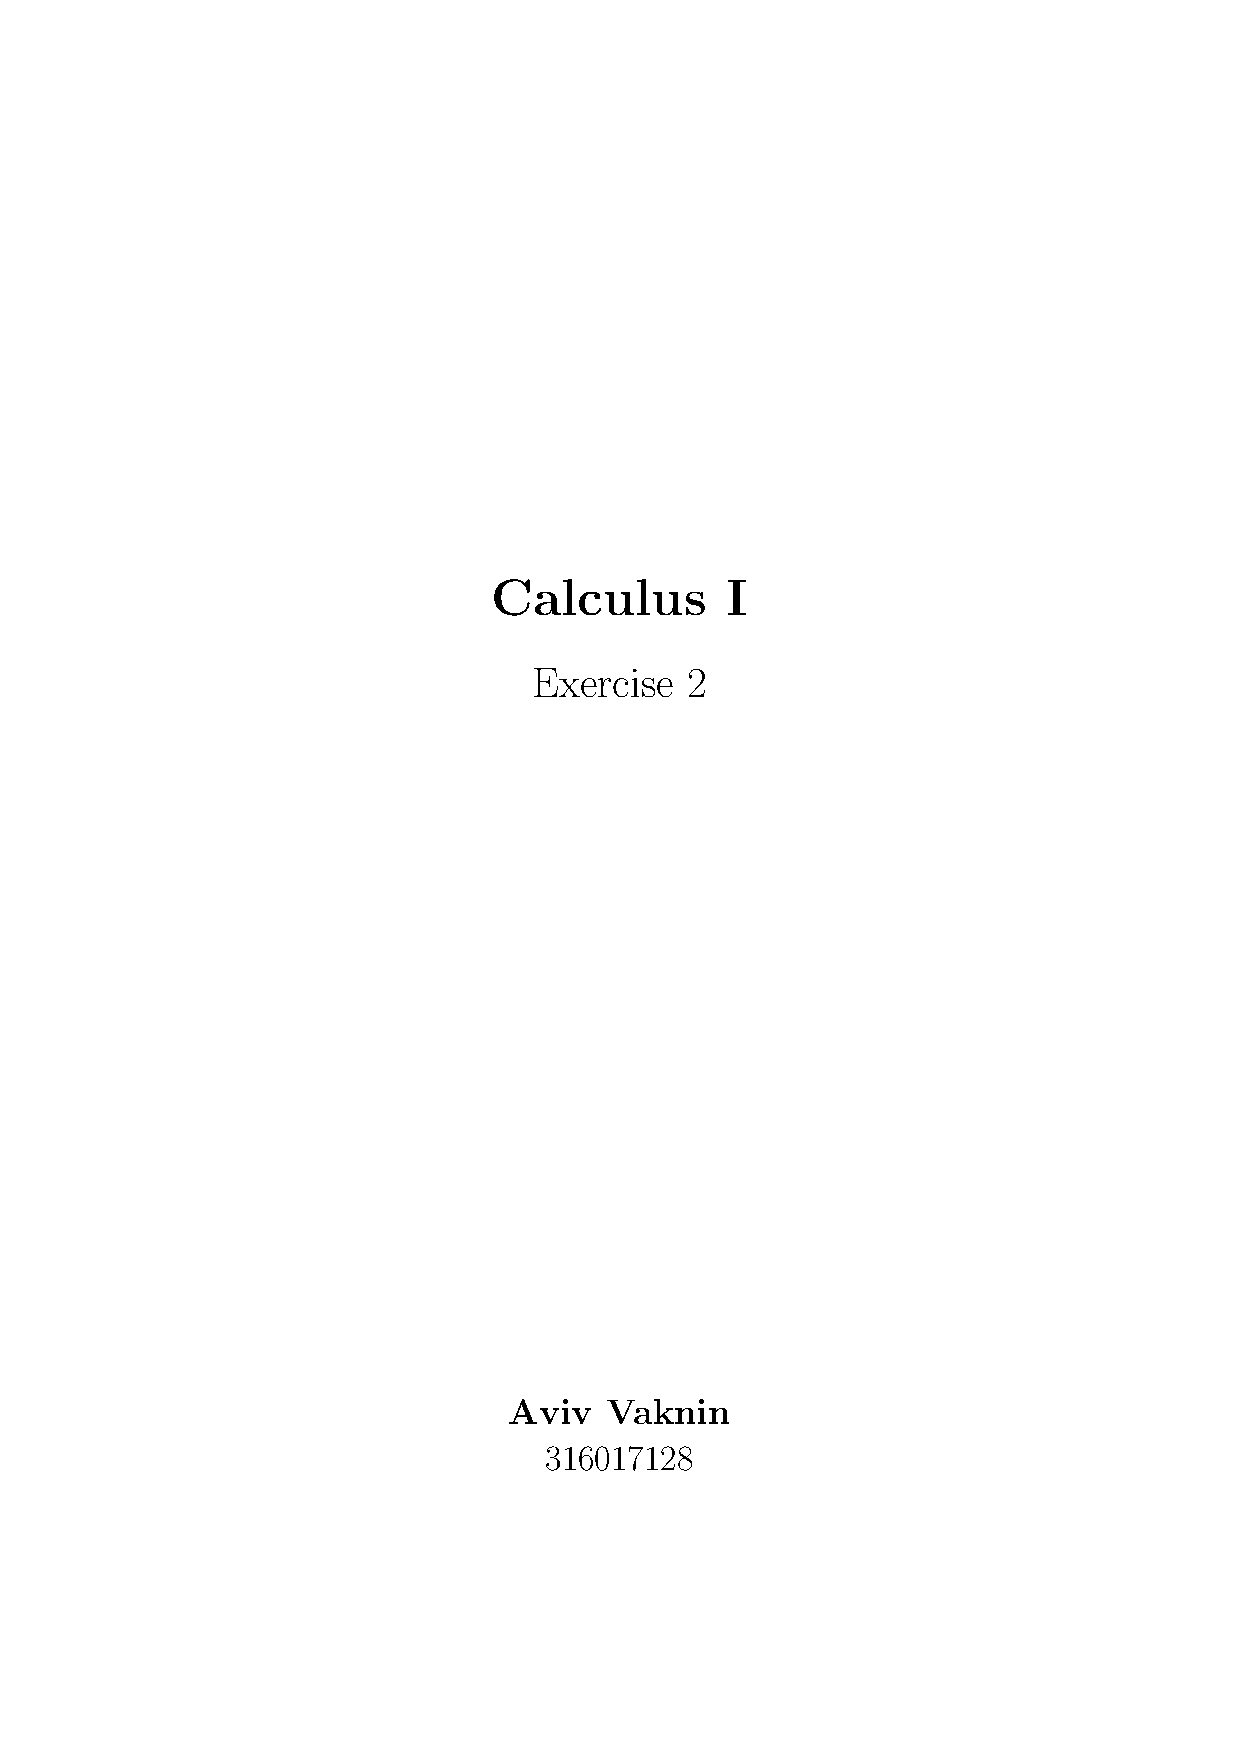
\includepdf{title.pdf}
\end{titlepage}

\section{Prove that \eq{a\leq{b} \iff \forall\epsilon>0~~a<b+\epsilon}}
\sub{$ a\leq{b} \Rightarrow \forall\epsilon>0~~a<b+\epsilon $:}
It is given that: \eq{0<\epsilon && a\leq{b}}
Therefore, because according to axiom $O3$ an ordered field is adhering to addition:
\eq{a+0<b+\epsilon}
It is worth mentioning that due to the uniqueness of zero, $b+\epsilon$ must be \textit{greater} than zero, rather than greater than or \textit{equal} to zero.
\sub{$ a\leq{b} \Leftarrow \forall\epsilon>0~~a<b+\epsilon $:}
We'll rephrase using contraposition: \eq{a>b \Rightarrow \exists\epsilon>0~~a\geq{b+\epsilon}}
We need to find an $\epsilon>0$ so that $a\geq{b+\epsilon}$.\\
Let $\epsilon=a-b$, now, we can see that:
\eq{
    b+\epsilon &= b+(a-b) = a\\
    a&\geq{b+\epsilon}
}
\qed

\section{Prove that \eq{\forall{m,n}\in{\F}~~mn\in{\F}}}
Let's assume that $m$ is some arbitrary natural number.\\
We'll prove using induction, starting with $n=1$:
According to axiom \textit{M3}:
\eq{m\cdot{1}=m}
It is given that $m\in{\F}$, therefore this case is valid.
Now, let's assume that it is true for a general $n$, i.e. $n=n$, and:
\eq{mn\in{\F}}
Now, we'll check $n=n+1$:
According to axiom \textit{D}:
\eq{ m(n+1)=mn+m }
We've assumed that $mn\in{\F}$, and it is given that $m\in{\F}$.\\
In addition, we've shown in exercise \textit{2a} that the natural numbers adhere to addition.\\
Therefore: \eq{mn\in{\F},~m\in{\F}\implies(mn+m)\in{\F}}
\qed

\section{Prove \eq{\sum^{n}_{k=1}k^{2}=\frac{n(n+1)(2n+1)}{6}}}
We'll prove this by induction:


% End
\end{document}